%% LyX 2.3.6 created this file.  For more info, see http://www.lyx.org/.
%% Do not edit unless you really know what you are doing.
\documentclass[a4paper,english]{scrartcl}
\usepackage[T1]{fontenc}
\usepackage[latin9]{inputenc}
\usepackage{amsmath}
\usepackage{graphicx}
\PassOptionsToPackage{normalem}{ulem}
\usepackage{ulem}

\makeatletter

%%%%%%%%%%%%%%%%%%%%%%%%%%%%%% LyX specific LaTeX commands.
\pdfpageheight\paperheight
\pdfpagewidth\paperwidth


\makeatother

\usepackage{babel}
\usepackage{listings}
\renewcommand{\lstlistingname}{Listing}

\begin{document}
\title{SEA3004F M3P1: Scalar and vector fields: coordinates and gradient}
\date{Ocean and Atmosphere Dynamics}
\maketitle

\section{Tutorial: Scalar fields from model data}

The aim of the tutorial is to familiarize with scalar and vector fields, i.e. arrays in geosciences. We will explore a scalar field representing mean sea level pressure values (the field is obtained from an atmospheric \emph{reanalysis} for the mean December 2014 conditions done by the
American National Center for Environmental Predictions). This is the
same figure shown in Sec. M3.1. We will not use a mapping package
to show the coastlines but the pressure field is exactly the same.
The data are stored in a file with the MATLAB format (.mat) (\texttt{NCEP\_slp\_matlab\_DXY.mat}).
We will also need the script \texttt{coloroposneg.m}. This special
function sets the ranges of the colorbar to show positive and negative
values (this function must be downloaded from vula; it isn't part
of matlab/octave, and therefore the file must be in the same directory
to be found).

As usual, first create a new directory on the computer, download the
files and work from that folder. Start a new Live Script and add the
following 

\begin{lstlisting}[language=Matlab,basicstyle={\small},showstringspaces=false,frame=lines]
% load the data into your workspace
load NCEP_slp_matlab_DXY 
% check the content of your workspace and size of the variables
whos
figure
% plot a pseudocolor map of the matrix: what do you see?
pcolor(slp201412)
% put the display in matrix mode (ij and not cartesian xy)
axis ij
\end{lstlisting}

The field is plotted using a ``matrix plane mode'', where x and
y correspond to the number of rows and columns. 

Fields in Earth Sciences should be presented on a \textbf{geographical
grid}. The \uline{coordinates are scalar fields as well}: every
element of the matrix indicate the latitude and longitude value of
that point. In the terminal window, first check the first elements
of your matrix:

\begin{lstlisting}[language=Matlab,basicstyle={\small},showstringspaces=false,frame=lines]
>> lon(1,1)   % check the value of lon and lat for the upper left corner
>> lat(1,1)
\end{lstlisting}

In the Live Script, test the following:

\begin{lstlisting}[language=Matlab,basicstyle={\small},showstringspaces=false,frame=lines]
figure     % graph a pseudocolor map of the scalar field "lon"
pcolor(lon)
colorposneg % this function changes the colors to show a pos/neg field
colorbar

% do the same for the latitude array in another code cell

% Plot the pressure field, now using the coordinates as the system of reference
figure
pcolor(lon,lat,slp201412)
xlabel('Longitude')
ylabel('Latitude')
colorbar
title('Mean sea level pressure 2014/12 (hPa)')
% print -dpng MSLP201412.png
\end{lstlisting}


\section{Tutorial: distances on a sphere}

To compute the vector operators on the Earth (\emph{gradient, divergence
and curl}) we \textbf{must} use distances expressed in metres, not
degrees. The \textbf{great circle} is the curve of least distance
on the surface of the sphere between any two points. When one travels
along meridians (all great circles), distances are always the shortest,
while travelling along parallels (only the Equator is a great circle)
leads to longer distances (Fig. 1). This implies that the length of
an arc of longitude changes with the latitude and we need to take
that into account when computing distances. The gradient, divergence
and curl operations are based on the \textbf{nabla} operator 
\[
\nabla\equiv\left(\frac{\partial}{\partial x},\:\frac{\partial}{\partial y},\:\frac{\partial}{\partial z}\right)
\]
and they all involve the computation of spatial differences.

\begin{figure}
\centering\includegraphics[scale=0.6]{great_circle-vs-rhumb_line}

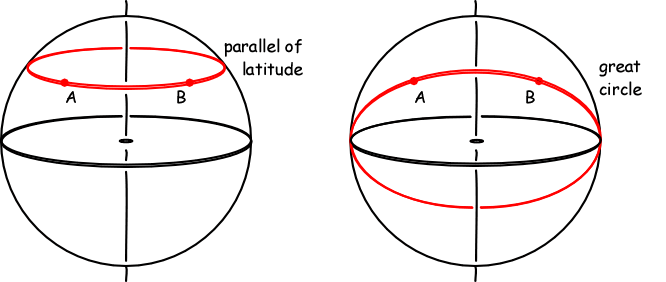
\includegraphics[scale=0.5]{parallel_orthodrome_loxodrome}

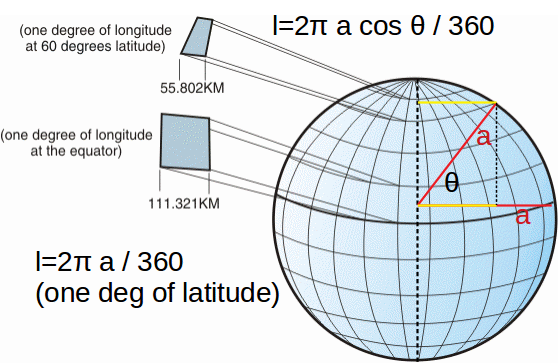
\includegraphics[scale=0.5]{longitude_latitude_edited}

\caption{Distances on a sphere. The distance on a great circle is called \textbf{orthodrome},
while the distance on constant bearing is called \textbf{loxodrome}
(or rhumb line). To calculate the length of one arc longitude at a
given latitude you need to compute the radius of the corresponding
circle.}
\end{figure}

We will practice this feature on the mean sea level pressure 

\begin{lstlisting}[language=Matlab,basicstyle={\small},showstringspaces=false,frame=lines]
load NCEP_slp_matlab_  % load the data into your workspace if not done

% In the terminal!
lon(1,1)   % check the value of lon and lat for the first element
lat(1,1)
dy=lat(1,1)-lat(2,1)  % check the delta of latitude 
dx=lon(1,2)-lon(1,1)  % check the delta of longitude 
DELTA = dx;

% Calculate distances on the sphere
% the arrays Xkm and Ykm in your workspace contain the km coordinates between
% the origin and every grid point at 2.5 deg lat and lon
figure
lims = [-20e3, 20e3]; % set the ranges of the color shading (km)
subplot(2,1,1) % create a subplot (2 rows, 1 column, 1st plot)
pcolor(lon,lat,Xkm)
axis tight
colorposneg
clim(lims)
colorbar
xlabel('Longitude')
ylabel('Latitude')
title('X coordinate')
subplot(2,1,2) % create a subplot (2 rows, 1 column, 2nd plot)
pcolor(lon,lat,Ykm)
axis tight
xlabel('Longitude')
ylabel('Latitude')
colorposneg
clim(lims)
colorbar
title('Y coordinate')

% The snippet below shows how I computed the arrays Xkm and Ykm
% based on the formulae shown on the figure
a= 6378; % appx earth radius in km
y=36:-1:-36;
x=-72:71;
[X,Y]=meshgrid(x,y);
Xkm=2.5*2*pi*a*cosd(lat).*X/360;
Ykm=2.5*2*pi*a*Y/360;
\end{lstlisting}
In this example we have also learned how to plot two panels on one
single figure with the command \texttt{subplot}.

The gradient of the pressure field is numerically computed using the
function \texttt{gradient}. Because of the matrix coordinate system,
the meridional gradient is computed from row 1 downward (row 1 corresponds
to latitude 90N). However, the geographical system is oriented upward;
therefore \textbf{we must change the sign of the meridional gradient
computed using the matrix orientation}. No need to change the sign
of the zonal gradient as the orientation is the same (left-right =
W-E).

\begin{lstlisting}[language=Matlab,basicstyle={\small},showstringspaces=false,frame=lines]
% COMPUTE THE GRADIENT using the function "gradient" and plot contourlines
[gslpx,gslpy]=gradient(slp201412,DELTA);
gslpy=-gslpy; % see the note above!
clevs = -4:4; % we will plot contours every 1 hPa/deg
figure
subplot(2,1,1)
contourf(lon,lat,gslpx,clevs)
axis tight 
xlabel('Longitude')
ylabel('Latitude')
colorposneg
colorbar
title('Zonal pressure gradient (hPa/deg)')
subplot(2,1,2) 
contourf(lon,lat,gslpy,clevs)
axis tight
xlabel('Longitude')
ylabel('Latitude')
colorposneg
colorbar
title('Meridional pressure gradient (hPa/deg)')
\end{lstlisting}



\section{Exercise 2: Pressure gradient using distance [30]}

The pressure gradients using degrees of latitude and longitude cannot be compared with each other because the length of one degree is different. 

You will compute and plot the pressure gradients in units of hPa/km and not hPa/deg. However, the Matlab function is not sophisticated enough, and the octave gradient function is better. You will find \texttt{gradient\_octave.m} in the list of available files for the practical. Check out the help of the gradient function to find out how to insert the matrix of coordinates. This is now a numerical gradient calculated according to a specific reference system.

Create another section of your Live Script to calculate and visualize the components of the gradient in a two-panel figure (2 rows, 1 column) using \texttt{pcolor}. Set the ranges with \texttt{clim} to have the same range of values in the colorbar for both plots (you will
need to first generate an autoscaled plot and then check what is the best range to visualize the values). 
\end{document}
